\documentclass[10pt]{beamer}

%%%
% PREAMBLE FOR THIS DOC 
%%%
%https://tex.stackexchange.com/questions/68821/is-it-possible-to-create-a-latex-preamble-header
\usepackage{/Users/miw267/Repos/csci246_fall2025/slides/preambles/beamer_preamble_for_CSCI246}


%%% TRY TO RESHOW TOC AT EACH SECTION START (with current section highlighted)
% Reference: https://tex.stackexchange.com/questions/280436/how-to-highlight-a-specific-section-in-beamer-toc
\newcommand\tocforsect[2]{%
  \begingroup
  \edef\safesection{\thesection}
  \setcounter{section}{#1}
  \tableofcontents[#2,currentsection]
  \setcounter{section}{\safesection}
  \endgroup
}


%%%% HERES HOW TO DO IT CORRECTLY
% FIRST IN .STY FILE, DO
%\usetheme[sectionpage=none]{metropolis}
% THEN AT EACH SECTION DO
%\begin{frame}{Outline}
%  \tableofcontents[currentsection]	
%\end{frame}



%\setbeamertemplate{navigation symbols}{}
%\setbeamertemplate{footline}[frame number]{}


%%%
% DOCUMENT
%%%

\begin{document}

%\maketitle

%% Title page frame
%\begin{frame}
%    \titlepage 
%\end{frame}





\title{09/03/2025: Boolean Algebra}
\author{CSCI 246: Discrete Structures}
\date{Textbook reference: Sec. 7, Scheinerman}

\begin{frame}
    \titlepage 
\end{frame}




\begin{frame}

\vfill 
\begin{mygreenbox}[title=Quiz return method]
Quizzes are grouped into four bins (A-G, H-L, M-R, S-Z) by last name. \\
The quizzes are upside down with your last name on the back. \\
Come find yours before, during, or after class. \\
Only turn the quiz over if it's yours.
\end{mygreenbox} 
\vfill 

\begin{myyellowbox}[title=Today's Agenda]
\begin{itemize}
	\item Review  ($\approx$ 10 mins)
	\item Boolean algebra ($\approx$ 10 mins)
	\item Group exercises ($\approx$ 15 mins)
	\item Review group exercises ($\approx$ 15 mins)	
\end{itemize}

\end{myyellowbox}
\end{frame}






\begin{frame}[standout]
Outline for today's material
\begin{itemize}
\item \textbullet \quad \alert{Review}
\item \textbullet \quad Boolean Algebra
\item \textbullet \quad Group exercises
\item \textbullet \quad Review group exercises
\end{itemize}

\end{frame}


\begin{frame}{Weekly Quiz \#1: Scores}

\begin{figure}[ht]
        \centering
        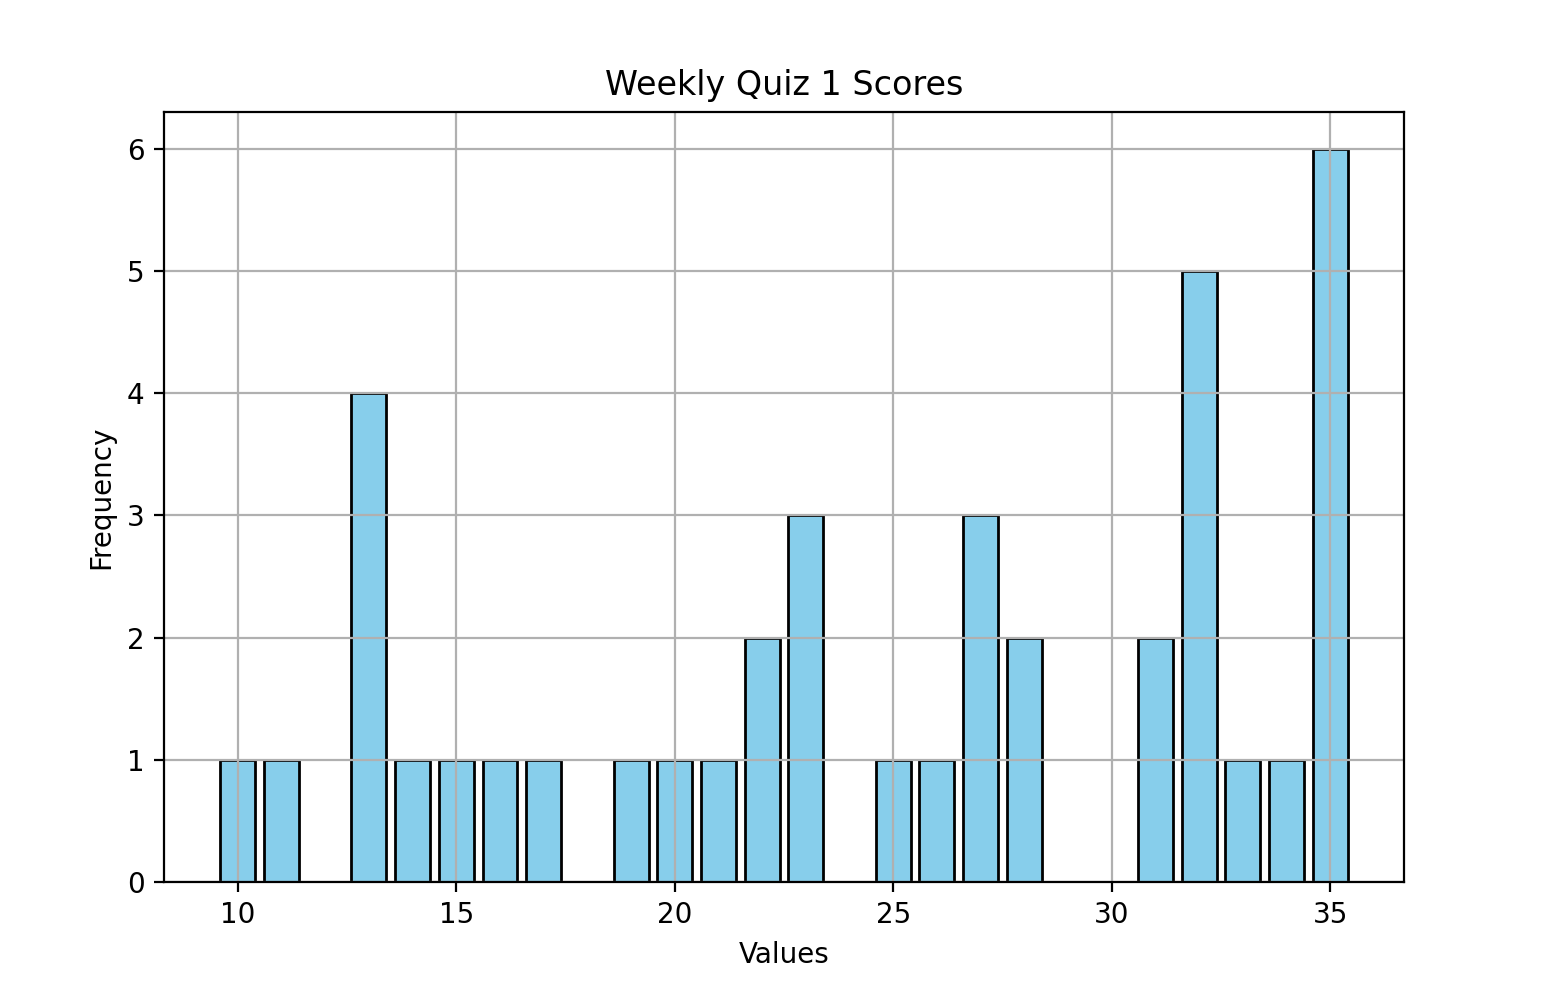
\includegraphics[width=\textwidth]{images/quiz1_scores}
        \caption{Reading Quiz Scores. Median: 26.5/35 (75.7\%)}
\end{figure}
\vfill 

\end{frame}


\begin{frame}{Review of Weekly Quiz \#1}

\begin{myredbox}[title=Reflections ($\approx$ 3 min)]
Take out a sheet of paper and tell me about your experience with the quiz -- How was it? \\

In particular, I'm interested in:
\begin{enumerate}
\item What can you do to help prepare yourself for future quizzes?	
\item What can I do to help prepare you for future quizzes?
\end{enumerate}
\end{myredbox}
			
\end{frame}


\begin{frame}{Study Guide For Quiz 2}


\begin{myredbox}[title=Readings (1 question)]
Sec. 6 (Counterexample)
\begin{itemize}
\item Know how to apply Proof Template 3.
\item In particular, know how to disprove Statement 6.1. 
\end{itemize}
Sec. 7 (Boolean Algebra)
\begin{itemize}
\item Know how to prove Props 7.1 and 7.3 using truth tables.
\item Understand the Boolean algebra properties listed in Theorem 7.2.  (What are they saying? Could you imagine proving them using truth tables?)
\end{itemize}

\end{myredbox}

\vfill 

\begin{myyellowbox}[title=Group exercises (2 questions)]
Know how to do all of the group exercises from these 2 sections.
\end{myyellowbox}

\end{frame}







\begin{frame}{Review of Sec. 6 (Counterexamples)}
\label{frame:assumption_not_met}
 \begin{mygreenbox}
Disprove the following conjecture:  
\textit{Let $a$ and $b$ be integers.  If $a|b$ and $b|a$, then $a=b$.}  
\end{mygreenbox}
\vfill 
\begin{myyellowbox}[title=Poll]
Is $a=1, b=0$ a valid counterexample?
\end{myyellowbox}
\vfill 
\pause 
	\begin{mydef}[title=Reminder of Definition 3.2 (\textbf{Divisible})]
	Let $a$ and $b$ be integers.  We say that $a$ is \textit{divisible} by $b$ provided there is an integer $c$ such that $bc=a$. The notation for this is $b|a$. 
	\end{mydef}
\vfill 	
\pause 
\footnotesize 
\textbf{Solution to poll:} The proposition $\red{a}|\blue{b} \; (= \red{1}|
\blue{0})$ is \texttt{true}, since there is an integer $\green{c}$ (namely $\green{c=0}$) such that $\red{a}\green{c}=\blue{b}$ (since $\red{1} \cdot \green{0} = \blue{0}$). However, the proposition $\blue{b}|\red{a} \; (= \blue{0}|\red{1})$ is \texttt{false}, since there is no integer $\purple{d}$ such that $\blue{b}\purple{d}=\red{a}$ (that is, there is no integer $\purple{d}$ such that  $\blue{0}\cdot \purple{d} = \red{1}$). Overall, \alert{the hypothesis doesn't hold, so we have not disproven the statement}.  
\end{frame}


\begin{frame}{Review of Sec. 6 (Counterexamples)}
\footnotesize 

 \begin{mygreenbox}
\footnotesize 
Disprove the following conjecture: \textit{Let $a$ and $b$ be integers.  If $a|b$ and $b|a$, then $a=b$.}
\end{mygreenbox}

\vfill 
\begin{myyellowbox}
Is $a=5, b=-5$ a valid counterexample? \pause  Yes it is!  See the proof below.
\end{myyellowbox}
\vfill 

\vfill \vfill 
\footnotesize 
%\textbf{Solution.} 

\begin{tabularx}{\textwidth}{|L{3cm}|X|}
\hline 
\onslide*<3->{\textbf{Annotation} & \textbf{Main Text}} \\ \hline
\onslide*<4->{\hlorange{Structure} & \hlorange{Let $a=5$, $b=-5$. First, we show that the hypothesis holds [i.e., that $(5|-5)$ and $(-5|5)$].}}  \\
\onslide*<5->{\hlgreen{Unravel defn.} & \hlgreen{$a|b$ means there is an integer $x$ such that $ax=b$. Likewise $b|a$ means there is an integer $y$ such that $by=a$.}} \\
\onslide*<6->{\hlred{The ``Glue"} & \hlred{Substituting for $a$ and $b$, we need to show that there are integers  $x$ and $y$ such that $5x=-5$ and $-5y=5$.   We see these equations hold by taking $x=-1$ and $y=-1$.}} \\
\onslide*<7->{\hlorange{Structure}  & \hlorange{Hence $5|-5$ and $-5|5$, so the hypothesis is met.}} \\
\hline
\onslide*<8->{\hlorange{Structure}  & \hlorange{Now we show that the conclusion fails [i.e. that $-5\neq5$.]}} \\
\onslide*<9->{\hlred{The ``Glue"} &  \hlred{This is immediately clear.}} \\
\hline
\end{tabularx}
\end{frame}



\begin{frame}{Review of Sec. 6 (Counterexamples)}

\begin{myyellowbox}[title=Poll]
Is the following statement true or false? 
\[ -5|5 = -1 \] 
\end{myyellowbox}

\pause 

\begin{myredbox}[title=Alert!]
In mathematical reasoning, you always need to \textbf{refer back to the definitions}.    
\end{myredbox}

\pause 
	\begin{mydef}[title=Reminder of Definition 3.2 (\textbf{Divisible})]
	Let $a$ and $b$ be integers.  We say that $a$ is \textit{divisible} by $b$ provided there is an integer $c$ such that $bc=a$. The notation for this is $b|a$. 
	\end{mydef}
\pause 
\footnotesize 
Solution to poll: The statement is \textbf{incorrect}! Why? \pause $-5|5$ is a \textbf{proposition}, so it can't equal $-1$. We would instead write just $-5|5$, or perhaps $-5|5 = \texttt{TRUE}$. %How do we justify the proposition? \pause We have $-5|5$ because if $a=5$ and $b=-5$, there exists an integer (namely $c=-1$) such that $bc=a$.
\end{frame}










\begin{frame}[standout]
Outline for today's material
\begin{itemize}
\item \textbullet \quad Review
\item \textbullet \quad \alert{Boolean Algebra}
\item \textbullet \quad Group exercises
\item \textbullet \quad Review group exercises
\end{itemize}

\end{frame}


\begin{frame}{Boolean algebra}

\begin{myyellowbox}[title=What is algebra?]
\textbf{Algebra} lets us reason about \alert{numbers}.  For example, using algebra, we can show that
\[ x^2 - y^2 = (x-y)(x+y) \]	
\end{myyellowbox}


\vfill 
\pause 

\begin{mygreenbox}[title=What is Boolean algebra?]
\textbf{Boolean Algebra} lets us reason about \alert{propositions}.   For instance, using Boolean Algebra, we can show that
\begin{itemize}
\item \texttt{If A, then B}	
\item \texttt{(not A) or B}
\end{itemize}
mean the same thing.
\end{mygreenbox}
\end{frame}

\begin{frame}{Reasoning about propositions}

\begin{myredbox}
To reason about propositions, we can use two tools:

\begin{itemize}
	\item Truth Tables
	\item Boolean Algebra Properties
\end{itemize}	
\end{myredbox}
\end{frame}

\begin{frame}{Tool \#1:  Truth Tables}
 \begin{mygreenbox}[title=Practice Reading Quiz (Sec. 7 - Boolean Algebra)]
Use a truth table to prove that the expressions $x \implies y$ and $(\lnot x) \, \lor \, y$ are logically equivalent.
\vfill 
\end{mygreenbox}
\vfill

\begin{myredbox}[title=Notation reminder]
\begin{itemize}
\item $\implies$ means \texttt{implies}
\item $\lnot$ means \texttt{not}
\item $\lor$ means \texttt{or} 	
\end{itemize}
\end{myredbox}
\vfill
\pause 
\colorbox{green!30}{\textbf{Solution.}}  The 3rd and 6th columns are the same.
\begin{center}
\begin{tabular}{ccc|ccc}
X & Y & $X \implies Y$ & $ \lnot X$  & $Y$   & $ (\lnot X) \lor Y$  \\
\hline 
T & T & T & F & T & T \\
T & F & F & F & F & F \\
F & T & T  &T &T & T \\
F & F & T  &T  &F & T \\
\end{tabular}
\end{center}	
\end{frame}


\begin{frame}{Tool \#2: Properties}
\footnotesize 


In the group exercises, we will see that we can also use the following properties to reason about propositions.
 
\vfill 
\begin{figure}[ht]
        \centering
        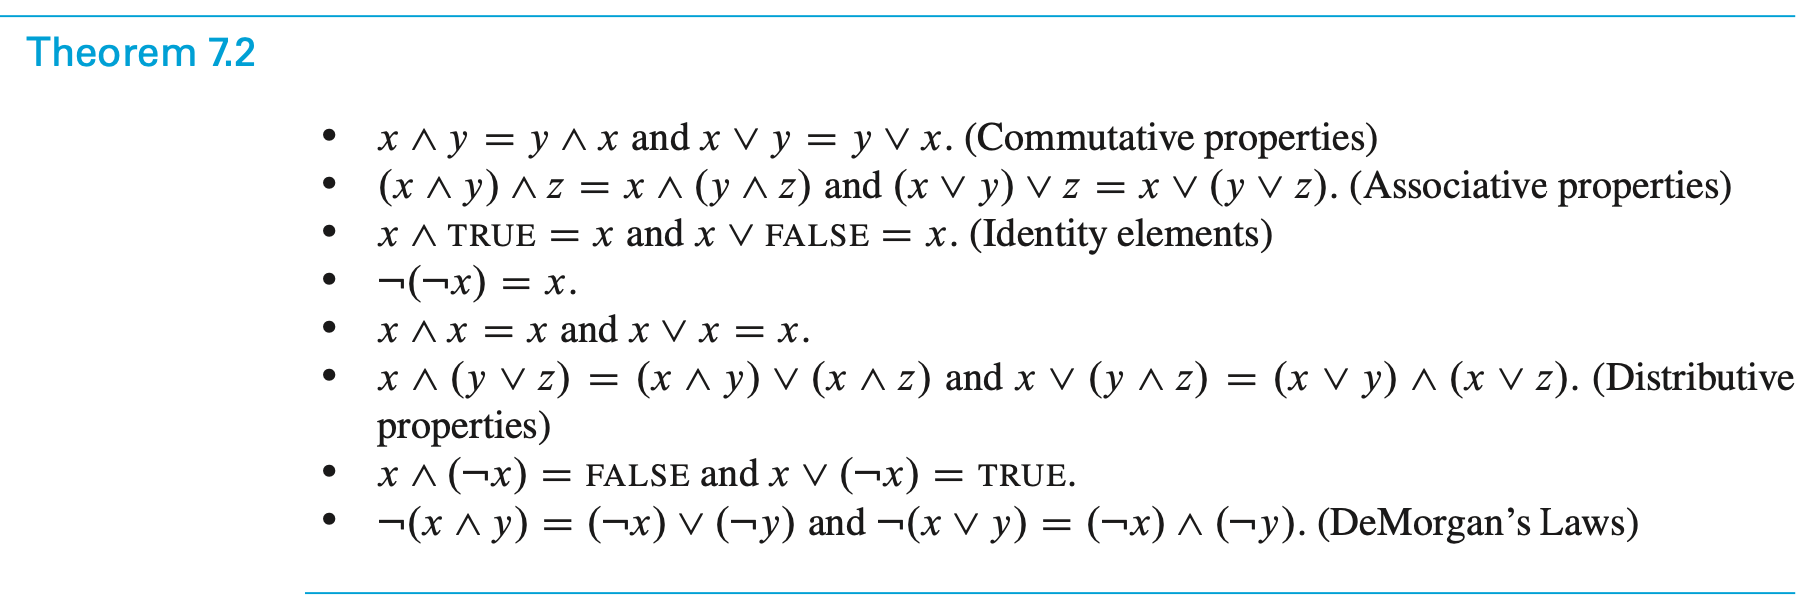
\includegraphics[width=\textwidth]{images/boolean_algebra_properties}
        \caption{Boolean Algebra Properties}
        \label{fig:bap}
\end{figure}
\vfill 
\pause 
These properties are proven via truth tables.   You can use them as \alert{shortcuts}.
\vspace{-.5cm}
\hfill 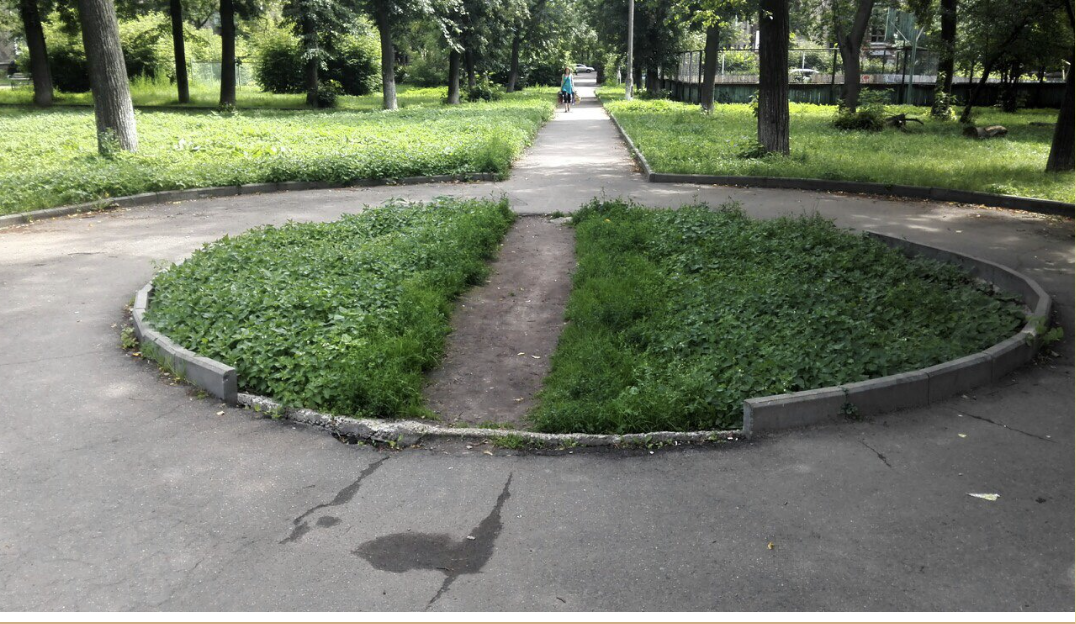
\includegraphics[height=2.5cm]{images/shortcut}.
\end{frame}

\begin{frame}{Boolean Algebra Properties: Example}

\begin{myredbox}[title=DeMorgan's Laws]
For propositions $P$ and $Q$:
\[ 1. \quad \lnot (P \land Q) = (\lnot P) \lor (\lnot Q) \qquad \qquad 2. \quad \lnot (P \lor Q) = (\lnot P) \land (\lnot Q)\]
\end{myredbox}

\vfill 

\only<1-2>{\begin{myyellowbox}[title=Poll]
How can we understand/interpret these?
\end{myyellowbox}
}

\vfill 
\pause 
\only<2>{\begin{mygreenbox}[title=Verbalization]
\begin{enumerate}
	\item 	\qq{Not (P and Q)} is the same as \qq{(Not P) or (Not Q).}
	\item \qq{Not (P or Q)} is the same as \qq{(Not P) and (Not Q).}
\end{enumerate}
\end{mygreenbox}}

\only<3>{\begin{mygreenbox}[title=Everyday example]
\footnotesize 
Suppose $P:$ Paul is at the party. $Q:$ Kunal is at the party.

\underline{Law 1}:
\begin{enumerate}
	\item \textbf{Left side}: \qq{It’s not true that Paul and Kunal are both at the party.}
	\item  \textbf{Right side}: \qq{Either Paul is not at the party, or Kunal is not at the party (or both).}
\end{enumerate}
\greencheck Same meaning! If they're not both there, then at least one of them must be absent.

\underline{Law 2}:
\begin{enumerate}
	\item \textbf{Left side}: \qq{It’s not true that Paul or Kunal is at the party..}
	\item  \textbf{Right side}: \qq{Paul is not at the party, and Kunal is not at the party.}
\end{enumerate}
\greencheck Again the same. If the party doesn’t have either one, then both must be absent.
\end{mygreenbox}}






\only<4>{\begin{mygreenbox}[title=Visual intuition]
\begin{center}
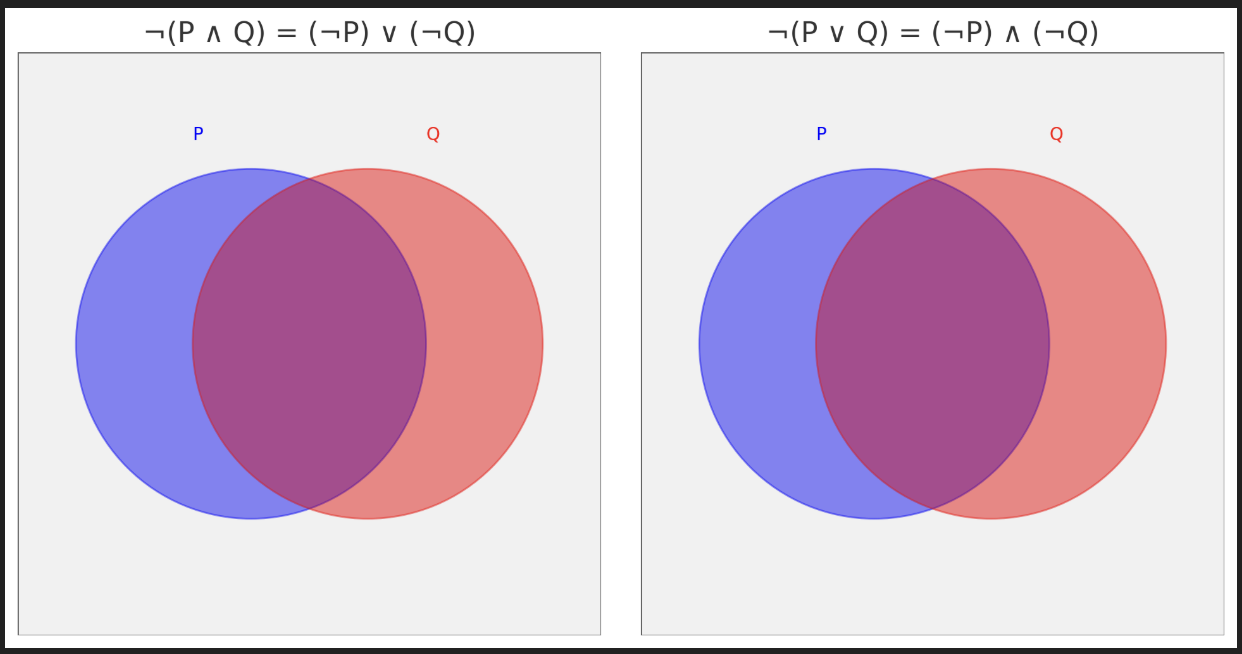
\includegraphics[width=.75\textwidth]{images/demorgan.png}
\end{center}
\footnotesize 
\vspace{-.4cm}
\begin{itemize}
	\item On the left,  $\lnot (P \land Q)$: everything except the overlapping middle part.
	\item On the right,  $\lnot (P \lor Q)$: everything outside both circles.
\end{itemize}

\end{mygreenbox}
}

\end{frame}


\begin{frame}[standout]
Outline for today's material
\begin{itemize}
\item \textbullet \quad Review
\item \textbullet \quad Boolean Algebra
\item \textbullet \quad \alert{Group exercises}
\item \textbullet \quad Review group exercises
\end{itemize}

\end{frame}


\begin{frame}{Random group assignments}
\footnotesize
\begin{columns}
\begin{column}{0.33\textwidth}
Aaron Christensen: 5 \\ 
Aidan Sinclair: 16 \\ 
Bennett Dijkstra: 7 \\ 
Brendan Kelly: 2 \\ 
Buggy Garza: 12 \\ 
Cedric Jefferson: 10 \\ 
Conner Brost: 17 \\ 
Connor Graville: 12 \\ 
David Knauert: 16 \\ 
David Oswald: 7 \\ 
Elias Martin: 8 \\ 
Ericson O'Guinn: 10 \\ 
Erik Halverson: 11 \\ 
Francis Bush: 5 \\ 
Garrett Miller: 6 \\ 
George Cutler: 14 \\ 
Georgia Franks: 12 \\ 
Gregor Schmidt: 8 \\\end{column}
\begin{column}{0.33\textwidth}
Hakyla Riggs: 5 \\ 
Izayah Abayomi: 3 \\ 
Jacob Ketola: 1 \\ 
Jacob Ruiz: 10 \\ 
Jaden Hampton: 15 \\ 
Jeremy Ness: 9 \\ 
Jonah Day: 15 \\ 
Karter Gress: 14 \\ 
Kyle Hoerner: 17 \\ 
Landry Clarke: 15 \\ 
Leon BirdHat: 8 \\ 
Lillian Ziegler: 11 \\ 
Matthew Rau: 11 \\ 
Matyas Kari: 4 \\ 
Micah Miller: 1 \\ 
Michael Pitman: 4 \\\end{column}
\begin{column}{0.33\textwidth}
Nathan Campbell: 2 \\ 
Nathan Hooley: 18 \\ 
Nicholas Rugani: 9 \\ 
Noah Andersson: 13 \\ 
Olivia Greuter: 16 \\ 
Peter Van Vleet: 14 \\ 
Pierce Dotson: 17 \\ 
Quinn Carlson: 7 \\ 
Ridley Christoferson: 2 \\ 
Riley Smith: 13 \\ 
Sierra Holleman: 6 \\ 
Tanner Gramps: 1 \\ 
Timothy True: 13 \\ 
Titus Sykes: 3 \\ 
Trey Randall: 4 \\ 
William Grant: 9 \\ 
William Sheldon: 3 \\ 
Zachary Reller: 6 \\\end{column}
\end{columns}
\end{frame}


\begin{frame}{Group exercises}
\footnotesize 
\begin{enumerate}
	\item DeMorgan's laws are:
	\[ \lnot (x \land y) = (\lnot x) \lor (\lnot y) \quad \text{and} \quad \lnot (x \lor y) = (\lnot x) \land (\lnot y) \]
	Prove the first of these (using truth tables). Then use DeMorgan's law to show how to disprove an if-and-only-if statement.
	\item A \textbf{tautology} is a Boolean expression that evaluates to \texttt{TRUE} for all possible values of its variables.  For example, the expression $x \lor \lnot x$ evaluates to \texttt{TRUE}  both when $x=\texttt{TRUE}$ and $x=\texttt{FALSE}$.  Use truth tables to show the following are tautologies:
	    \vspace{-0.5cm}
		\begin{enumerate}
		\item[(a)] $(x \lor y) \lor (x \lor \lnot y)$
		\item[(b)] $x \implies x$
		\item[(c)] $\texttt{FALSE} \implies x$
		\item[(d)] $(x \implies y) \land (y \implies z) \implies (x \implies z)$ 
		\end{enumerate}
	\item  A \textbf{contradiction} is a Boolean expression that evaluates to \texttt{FALSE} for all possible values of its variables.  For example, the expression $x \land \lnot x$ is a contradiction.  Use truth tables to show that the following are contradictions:
		\begin{enumerate}
		\item[(a)] $(x \lor y) \land (x \lor \lnot y) \land \lnot x$
		\item[(b)] $x \land (x \implies y) \land (\lnot y)$.
		\end{enumerate}
	\item Reprove the items in \#2 and \#3 using the properties in Theorem 7.2 and the fact  from Prop 7.3 that $x \implies y$ is equivalent to $(\lnot x) \lor y$.
\end{enumerate}
\end{frame}

\begin{frame}[standout]
Solutions to group exercises	
\end{frame}

\begin{frame}{Solution to group exercise \#1a}
\textbf{Problem.} DeMorgan's laws are:
	\[ \lnot (X \land Y) = (\lnot X) \lor (\lnot Y) \quad \text{and} \quad \lnot (X \lor Y) = (\lnot X) \land (\lnot Y) \]
	Prove the first of these (using truth tables).  \\
	
\textbf{Solution.} 
\begin{center}
\begin{tabular}{cc|cc|ccc}
X & Y & $X \land Y$ & $ \lnot (X \land Y)$  & $ \lnot X$   & $ \lnot Y$  & $ (\lnot X) \lor (\lnot Y)$  \\
\hline 
T & T & T & F & F & F & F\\
T & F & F &T & F & T & T\\
F & T & F  &T &T & F & T \\
F & F & F  &T  &T & T & T\\
\end{tabular}
\end{center}	

The 4th and 7th columns have the same truth values.  Hence, $ \lnot (X \land Y) = (\lnot X) \lor (\lnot Y)$. 
\end{frame}



\begin{frame}{Solution to group exercise \#1b}
\small 

\textbf{Problem.} 
Use DeMorgan's law to show how to disprove an if-and-only-if statement.


\textbf{Solution.} In Group Exercise \#2 from the Theorems day, we showed that
%
\begin{align}
 A \iff B  \quad  = \quad (A \implies B) \land (B \implies A).
 \label{eqn:iff_equality}
\end{align}
%
That is, A-if-and-only-if B is identical to if-A-then-B \texttt{and} if-B-then-A.
\vfill 
To \alert{disprove} an if-and-only-if statement, we need to establish $\lnot (A \iff B)$.  Now note that:
%
\begin{align*}
\lnot (A \iff B) & = \lnot \bigg((A \implies B) \land (B \implies A)  \bigg) && \scripttext{(by substituting \Eqref{eqn:iff_equality})}. \\
&=  \lnot  (A \implies B) \lor  \lnot (B \implies A)  && \scripttext{(by DeMorgan's law)}
\end{align*}
 %
So we can disprove and if-and-only-if statement \textit{either} by showing that $A \implies B$ fails \textit{or} by showing that $B \implies A$ fails.  

\end{frame}

\begin{frame}{Solution to group exercise \#2a}
\textbf{Problem.} Use truth tables to show the following is a  tautology:
\[ (X \lor Y) \lor (X \lor \lnot Y) \]
\vfill 
\textbf{Solution.}
\begin{center}
\begin{tabular}{ccc|cc|c}
X & Y & $\lnot Y$ & $X \lor Y$ & $ X \lor (\lnot Y)$  & $ \big(X \lor Y\big) \lor \big(X \lor \lnot Y \big)$    \\
\hline 
T & T & F & T & T & T \\
T & F & T &T & T & T \\
F & T & F  &T &F & T \\
F & F & T  &F  &T & T \\
\end{tabular}
\end{center}

The last column shows that $ (X \lor Y) \lor (X \lor \lnot Y)$ is always true, and hence a tautology. 
\end{frame}


\begin{frame}{Solution to group exercise \#2b}
\textbf{Problem.} Use truth tables to show the following is a tautology:
\[X \implies X.\]
\vfill 
\textbf{Solution.}
Recall the truth table for implication. 
\begin{center}
\begin{tabular}{ccc}
X & Y & $X \implies Y$   \\
\hline 
T & T & T \\
T & F & F\\
F & T & T  \\
F & F & T  \\
\end{tabular}
\end{center}

Here we have Y=X.  So only the first and last row of the truth table ever occur.  So  $X \implies X$ is always true.  Thus,  $X \implies X$ is a tautology.
\end{frame}


\begin{frame}{Solution to group exercise \#2\,c}
\textbf{Problem.} Use truth tables to show the following is a tautology:
\[ \texttt{FALSE} \implies X\]
\vfill 
\textbf{Solution.}
The truth table for implication is
\begin{center}
\begin{tabular}{ccc}
W & X & $W \implies X$   \\
\hline 
T & T & T \\
T & F & F\\
F & T & T  \\
F & F & T  \\
\end{tabular}
\end{center}

But here, we know $W$ is \texttt{FALSE}.  That is, only the last two rows of the truth table ever occur.  So  $\texttt{FALSE} \implies X$ is always true.  Hence,  $\texttt{FALSE} \implies X$ is a tautology. 
\end{frame}

\begin{frame}{Solution to group exercise \#2\,d}
\footnotesize 
\textbf{Problem.} Use truth tables to show the following is a tautology:
\[ (X \implies Y) \land (Y \implies Z) \implies (X \implies Z) \]

\vfill 
\textbf{Solution.}
\begin{table}[h]
    \centering
    \begin{tabular}{cc|c c c c |c c c c}
        %\multirow{2}{*}{\textbf{Score}} & \multirow{2}{*}{\textbf{Frequency}} & 
        \toprule 
        \textbf{Proposition} & \textbf{Nickname} & \multicolumn{8}{c}{\textbf{Values}} \\
        \midrule
        X &&T&T&F&F&T&T&F&F \\
        Y &&T&F&T&F&T&F&T&F \\
        Z && \multicolumn{4}{c}{\cellcolor[gray]{0.9} T} &  \multicolumn{4}{c}{ \cellcolor[gray]{0.7} F}\\  
        \midrule
        $X \implies Y$&A &T&F&T&T&T&F&T&T \\
        $Y \implies Z$&B &\multicolumn{4}{c}{\cellcolor[gray]{0.9} T}&F&T&F&T \\
        $(X \implies Y) \land (Y \implies Z)$ &$C \defeq A \land B$ &T&F&T&T&F&F&F&T \\
        $X \implies Z$ &D &\multicolumn{4}{c}{\cellcolor[gray]{0.9} T} & F & F & T & T \\
         \tiny $(X \implies Y) \land (Y \implies Z) \implies (X \implies Z)$ &$C \implies D$&\multicolumn{4}{c}{\cellcolor[gray]{0.9} T} &  \multicolumn{4}{c}{ \cellcolor[gray]{0.7} T}\\
        \bottomrule
    \end{tabular}
\end{table}	
\end{frame}

\begin{frame}{Solution to group exercise \#3a}
\footnotesize 
\textbf{Problem.} Use truth tables to show the following is a contradiction:
\[ (X \lor Y) \land (X \lor \lnot Y) \land \lnot X \]

\vfill 
\textbf{Solution.}
\begin{table}[h]
    \centering
    \begin{tabular}{c | c|c c c c}
        \toprule 
        \textbf{Proposition} & \textbf{Nickname}& \multicolumn{4}{c}{\textbf{Truth Values}} \\
        \midrule
        X &&T&T&F&F\\
        Y &&T&F&T&F\\ 
        \midrule
        $X \lor Y$&A&T&T&T&F\\
        \midrule 
        $\lnot Y$ &&F&T&F&T \\
        $X \lor (\lnot Y)$&B &T&T&F&T \\
        \midrule 
        $\lnot X$&C &F&F&T&T \\
        $(X \lor Y) \land (X \lor \lnot Y) \land \lnot X$ & $A \land B \land C$ &F&F&F&F \\
        \bottomrule
    \end{tabular}
\end{table}	
\end{frame}

\begin{frame}{Solution to group exercise \#3b}
\footnotesize 
\textbf{Problem.} Use truth tables to show the following is a contradiction:
\[ X \land (X \implies Y) \land (\lnot Y) \]

\vfill 
\textbf{Solution.}
\begin{table}[h]
    \centering
    \begin{tabular}{c | c|c c c c}
        \toprule 
        \textbf{Proposition} & \textbf{Nickname}& \multicolumn{4}{c}{\textbf{Truth Values}} \\
        \midrule
        X &A&T&T&F&F\\
        Y &&T&F&T&F\\ 
        \midrule
        $X \implies Y$&B&T&F&T&T\\
        $\lnot Y$ &C &F&T&F&T \\
        \midrule 
        $X \land (X \implies Y) \land (\lnot Y)$ & $A \land B \land C$ &F&F&F&F \\
        \bottomrule
    \end{tabular}
\end{table}	
\end{frame}


\begin{frame}{Solution to group exercise \#4}
\footnotesize 

The solutions to group exercise \#4 refer to the properties from the textbook below. 
\vfill 
\begin{figure}[ht]
        \centering
        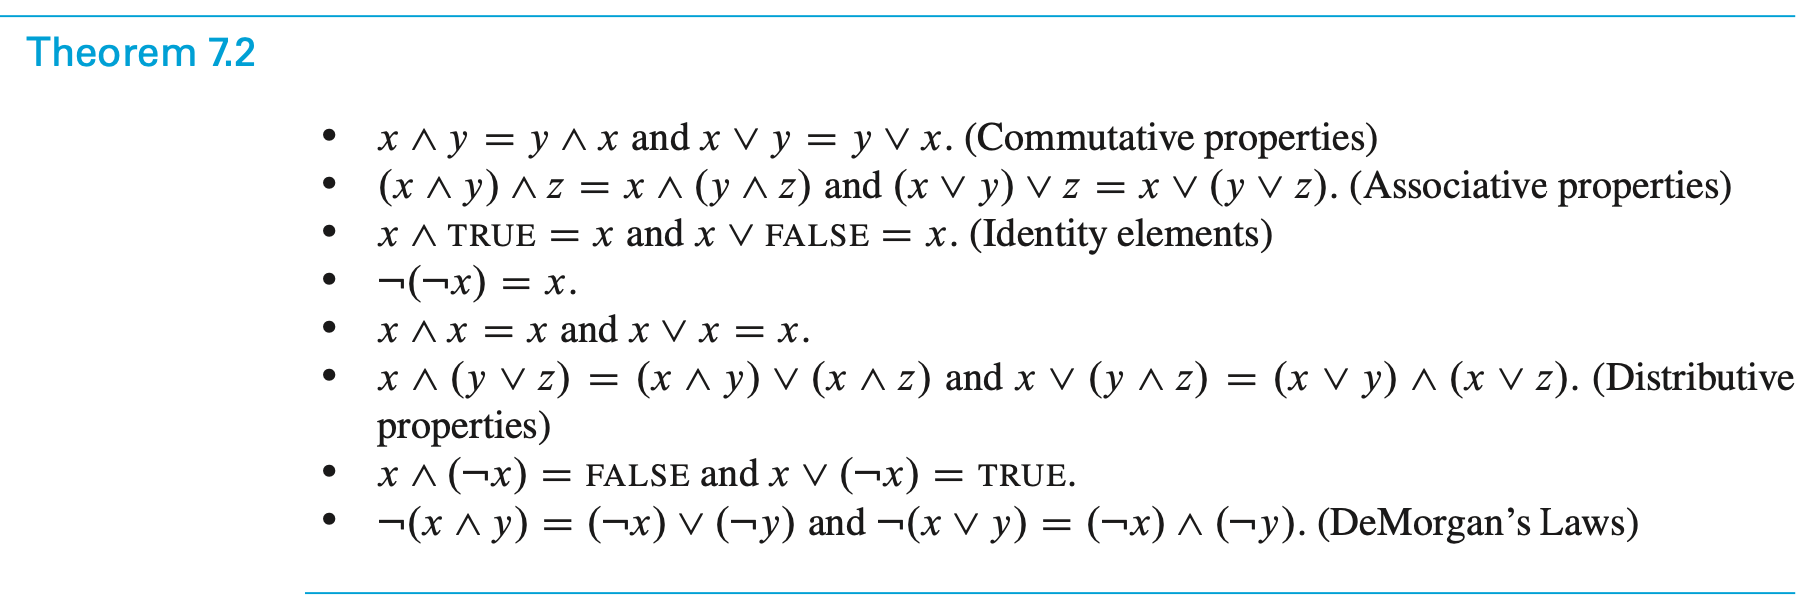
\includegraphics[width=\textwidth]{images/boolean_algebra_properties}
        \caption{Boolean Algebra Properties}
        \label{fig:bap}
\end{figure}
\end{frame}

\begin{frame}{Solution to group exercise \#4 - Redo of 2a}

\textbf{Problem.} Show the following is a  tautology:
\[ (X \lor Y) \lor (X \lor \lnot Y) \]
\vfill 
\textbf{Solution.}

\begin{align*}
(X \lor Y) \lor (X \lor \lnot Y) &= 	(X \lor X) \lor (Y \lor \lnot Y) && \scripttext{(commutative, associative props.)} \\
&= X \lor \texttt{True} && \scripttext{(unnamed props \#5,7)} \\
&= \texttt{True} && \scripttext{(unnamed prop \#7)}
\end{align*}

\end{frame}
		

\begin{frame}{Solution to group exercise \#4 - Redo of  \#2b}
\textbf{Problem.} Show the following is a tautology:
\[X \implies X.\]
\vfill 
\textbf{Solution.}
\begin{align*}
X \implies X  &= 	(\lnot X \lor X) && \scripttext{(Prop 7.3)} \\
&= \texttt{True} && \scripttext{(unnamed prop \#7)} 
\end{align*}

\end{frame}


\begin{frame}{Solution to group exercise \#4 - Redo of  \#2\,c}
\textbf{Problem.} Show the following is a tautology:
\[ \texttt{FALSE} \implies X\]
\vfill 
\textbf{Solution.}
%
\begin{align*}
\texttt{FALSE} \implies X  &= 	(\lnot \texttt{FALSE}) \lor X && \scripttext{(Prop 7.3)} \\
&= \texttt{TRUE} \lor X \\
&= \texttt{TRUE}
\end{align*}
\end{frame}

\begin{frame}{Solution to group exercise \#4 - Redo of  \#2\,d}
\footnotesize 
\textbf{Problem.} Show the following is a tautology:
\[ (X \implies Y) \land (Y \implies Z) \implies (X \implies Z) \]

\vfill 
%
\begin{align*}
& \explaintermbrace{$\defeq A$}{(X \implies Y) \land (Y \implies Z)} \implies \explaintermbrace{$\defeq B$}{(X \implies Z)} \\
=& \lnot A \lor B  && \scripttext{(Prop 7.3)}  \\
=& \bigg(  \lnot \big[X \implies Y \big] \lor \big[\lnot (Y \implies Z)\big] \bigg) \lor (X \implies Z)  && \scripttext{(DeMorgan's Law)}  \\
=& (X \lor \lnot Y) \lor (Y \lor \lnot Z) \lor (\lnot X \lor Z) && \scripttext{(Prop 7.3, DeMorgan's Law)}  \\
=& (X \lor \lnot X) \lor (Y \lor \lnot Y) \lor (Z \lor \lnot Z) && \scripttext{(Associative, commutative props.)}  \\
=& \texttt{TRUE}  \lor \texttt{TRUE}\lor \texttt{TRUE} && \scripttext{Unnamed Prop \#7} \\
=& \texttt{TRUE}
\end{align*}
%
\end{frame}

\begin{frame}{Solution to group exercise \#4 - Redo of  \#3a}
\footnotesize 
\textbf{Problem.} Show the following is a contradiction:
\[ (X \lor Y) \land (X \lor \lnot Y) \land \lnot X \]

\vfill 
\textbf{Solution.}
\begin{align*}
& (X \lor Y) \land (X \lor \lnot Y) \land \lnot X \\
=& (X \land X \land \lnot X) \lor (X \land \lnot Y \land \lnot X) \lor (Y \land X \land \lnot X) \lor (Y \land \lnot Y \land \lnot X) && \scripttext{Distributive prop.} \\
=& \texttt{FALSE} \lor \texttt{FALSE} \lor  \texttt{FALSE} \lor  \texttt{FALSE}  && \scripttext{Unnamed prop. \# 7} \\
=& \texttt{FALSE}
\end{align*}
\vfill 
\vfill
\begin{myredbox}[title=Remark]
A tricky part of applying the properties is using the distributive law correctly.  For intuition, recall how multiplication distributes over addition [e.g. $4(3+5) = 4 \cdot 3 + 4 \cdot 5$]. 
\end{myredbox}

\end{frame}

\begin{frame}{Solution to group exercise \#4 - Redo of  \#3b}
\footnotesize 
\textbf{Problem.} Show the following is a contradiction:
\[ X \land (X \implies Y) \land (\lnot Y) \]

\vfill 
\textbf{Solution.}
\begin{align*}
& X \land (X \implies Y) \land (\lnot Y) \\
=& 	 X \land (\lnot X \lor Y) \land (\lnot Y) && \scripttext{Prop 7.3} \\
=& (X \land \lnot X \land \lnot Y) \lor (X \land Y \land \lnot Y) && \scripttext{Distributive prop.} \\
=& \texttt{FALSE} \lor \texttt{FALSE} && \scripttext{Unnamed prop. \# 7} \\
=& \texttt{FALSE}
\end{align*}
\end{frame}


\end{document}
